\documentclass{article}

\usepackage[utf8]{inputenc}
\usepackage[dvipsnames]{xcolor}
\usepackage{lmodern}
\usepackage{graphicx}
\usepackage{longtable}
\usepackage{tabularx}
\graphicspath{ {../images/} }
\usepackage{imakeidx}
\makeindex[columns=3, title=Alphabetical Index, intoc]

\usepackage{tabularx}
\usepackage{amsmath}
\usepackage{paralist}
\usepackage{enumitem}
\usepackage{hyperref} %\usepackage[hidelinks]{hyperref} %per togliere bordi rossi
\usepackage{makecell}
\usepackage{caption}
\usepackage[maxfloats=256]{morefloats}
\maxdeadcycles=1000

\usepackage[official]{eurosym}
\DeclareUnicodeCharacter{20AC}{\euro{}}

\author{Agosta, Belli, Emili, Giacchini, Luciani}

\begin{document}

\begin{center}
    \sffamily{\fontsize{50}{48} \selectfont \textcolor{red}{Nexi}\textcolor{green}{Fy}}
\end{center}

\begin{center}
    \itshape{\fontsize{20}{48} \selectfont streaming to your pocket}
\end{center}

\bigskip\bigskip\bigskip

\begin{flushleft}
    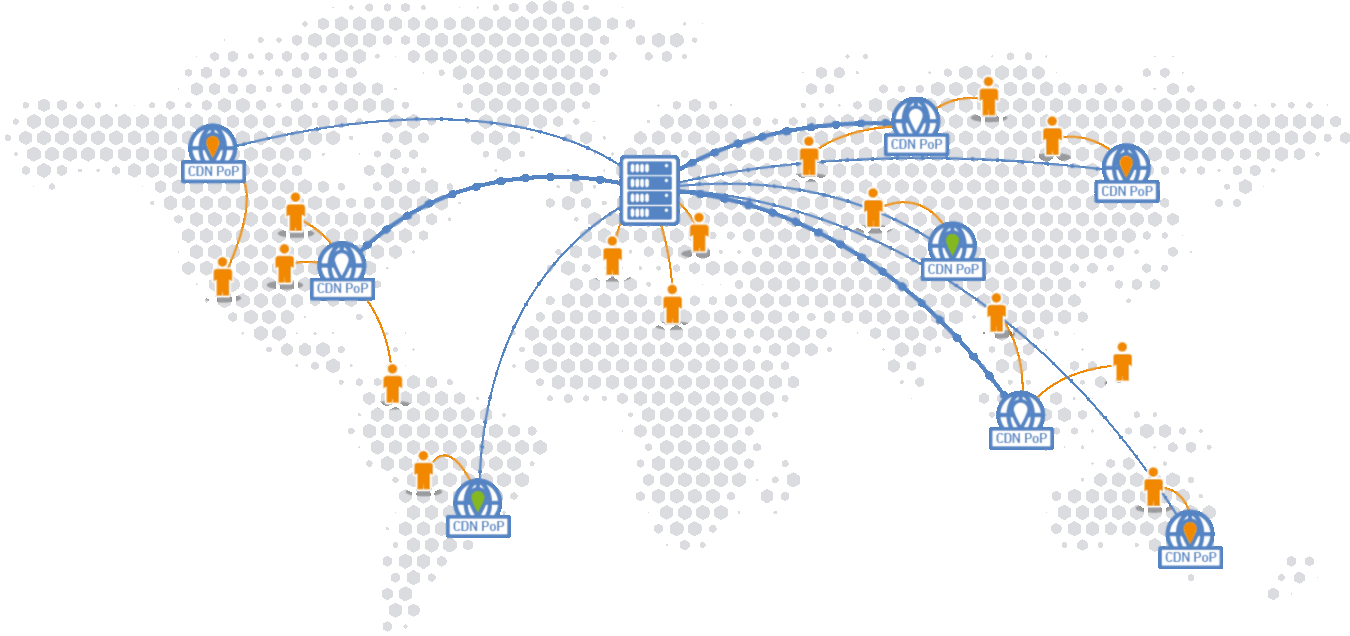
\includegraphics[scale=1]{../images/worldCDN.png}
\end{flushleft}

\bigskip\bigskip\bigskip

\begin{center}
    \itshape{\fontsize{30}{48} \selectfont Visione Del Sistema}
\end{center}

\newpage
\printindex

\newpage
\section{\itshape{Visione del Sistema}}
\textbf{NexiFy} è una piattaforma di streaming multimediale on demand che offre contenuti quali film, serie tv, brani e video musicali e altre forme di intrattenimento. Il servizio è fruibile sia via web che da app mobile.\\

La fruizione dei contenuti avviene attraverso un singolo player audio / video:
\begin{itemize}\item per la riproduzione di film o serie tv entrambe le tracce video e audio vengono riprodotte in contemporanea. L’utente può scegliere la qualità di riproduzione, manualmente o automaticamente, in base alle sue preferenze e disponibilità di connessione a internet. Possono essere mostrati anche dei sottotitoli (se disponibili).
    \item per la riproduzione di musica ci sono due scenari diversi (in entrambi i casi il brano può essere ascoltato con l’app in background, inibendo quindi la traccia video) :
    \begin{enumerate}
        \item il brano è accompagnato dal relativo video musicale; in questo caso vengono riprodotte entrambe le tracce audio e video contemporaneamente.
        \item il brano non è accompagnato dal video musicale; in questo caso viene riprodotta la sola traccia audio e al posto della traccia video, viene mostrata la copertina dell’album relativo al brano oppure i lyrics del brano in tempo reale (in base alla scelta dell’utente e alla disponibilità dei lyrics).
    \end{enumerate}
\end{itemize}
    
Gli utenti della piattaforma si dividono in due categorie: partner e iscritti.\\

I contenuti sono caricati da partner che sottoscrivono un contratto di collaborazione, pagando una quota annuale uguale per tutti ma modificabile nel corso del tempo. Questi ultimi ricevono un compenso in base al numero di riproduzioni che hanno ottenuto sui loro contenuti.\\

Gli iscritti sono coloro che usufruiscono del servizio; essi hanno la possibilità di scegliere diversi profili di abbonamento definibili a piacere tramite apposite funzioni di creazione a associazione degli abbonamenti alle varie funzionalità offerte dal sistema.\\

Questo servizio dà la possibilità agli iscritti interessati di visualizzare film e serie tv e ascoltare brani musicali sottoscrivendo un singolo abbonamento. Questo porta ad essi un risparmio di denaro, in quanto non è necessario iscriversi a diversi servizi il cui costo totale ammonterebbe ad una quota mensile maggiore.\\

\subsection{\itshape{Vincoli}}
NexiFy si riserva la possibilità di rimuovere qualsiasi contenuto video e/o audio presente sulla piattaforma che, dopo previa verifica, non rispetta la linee guida dei TOS.
In particolare è vietato il caricamento di qualsiasi traccia audio/video con contenuti sessualmente espliciti o che promuovono o giustificano l'uso della violenza contro persone o gruppi in base a razza, etnia, religione, disabilità fisiche, sesso, età, nazionalità né contenuti il cui scopo sia l'incitamento all'odio sulla base di tali caratteristiche.

\index{Index}

\subsection{\itshape{Configurazione del Sistema alla Consegna}}
Alla consegna del sistema prevediamo, già inclusi in esso, i seguenti abbonamenti designati e pensati per gli utenti:
\begin{itemize}
    \item Free (0 € / mese ) che darà accesso alle seguenti funzioni: 
	\begin{itemize}
   		\item Ascoltare brani musicali presenti sulla piattaforma \textbf{con} limiti di scelta di riproduzione e intermezzi pubblicitari;
		\item Visionare episodi pilota di serie tv;
		\item Visionare trailer di film.
	\end{itemize}
    \item Music (9.99 € / mese) che darà accesso alle seguenti funzioni:
	\begin{itemize}
   		\item Ascoltare brani musicali presenti sulla piattaforma \textbf{senza} limiti di scelta di riproduzione e intermezzi pubblicitari;
		\item Scaricare su dispositivo, tramite app mobile, brani musicali per usufruirne offline;
		\item Visionare episodi pilota di serie tv;
		\item Visionare trailer di film.
	\end{itemize}
    \item Premium (14.99 € / mese) che darà accesso alle seguenti funzioni:
	\begin{itemize}
   		\item Ascoltare brani musicali presenti sulla piattaforma \textbf{senza} limiti di scelta di riproduzione e intermezzi pubblicitari;
		\item Scaricare su dispositivo, tramite app mobile, brani musicali per usufruirne offline;
		\item Visionare tutti gli episodi delle serie tv presenti sulla piattaforma;
		\item Scaricare su dispositivo, tramite app mobile, episodi di serie tv per usufruirne offline;
		\item Visionare tutti i film presenti sulla piattaforma.
		\item Scaricare su dispositivo, tramite app mobile, film per usufruirne offline;
	\end{itemize}
	
	\item Partner (300 € / anno) che darà accesso alle seguenti funzioni:
	\begin{itemize}
   		\item Pubblicazione di video
		\item Pubblicazione di brani musicali
		\item Modifica/rimozione di video
		\item Modifica/rimozione di brani musicali
		\item Ricevere pagamenti in base alle visualizzazioni sui propri contenuti
	\end{itemize}
\end{itemize}


La CDN fornita coprirà l’intera area geografica globale arrivando in tempi ragionevoli a tutti gli utenti. Inoltre supporterà un numero massimo di XXXX utenti.


\index{Index}

\subsection{\itshape{Vincoli}}
\begin{itemize}
\item NexiFy si riserva di modificare la quota annuale per i partner.
\item NexiFy si riserva di rimuovere ogni contenuto considerato non idoneo ad essere visualizzato o riprodotto dagli utenti.
\item In caso di contenuti particolari, prima della riproduzione l'utente verrà informato, dando la possibilità di evitare contenuti non desiderati.
\item In particolare è vietato il caricamento di qualsiasi traccia audio/video con contenuti sessualmente espliciti o che promuovono o giustificano l'uso della violenza contro persone o gruppi in base a razza, etnia, religione, disabilità fisiche, sesso, età, nazionalità né contenuti il cui scopo sia l'incitamento all'odio sulla base di tali caratteristiche. 
\item NexiFy può creare/modificare/rimuovere profili di abbonamento. 
\item Qualsiasi risorsa audio o video scaricata tramite l'app mobile sarà codificata in modo tale da rendere il file accessibile \textbf{solo ed esclusivamente} tramite il player dell'app stessa onde evitare una riproduzione non consentita di questi.
\end{itemize}
 


\index{Index}

\end{document}
